%%%%%%%%%%%%%%%%%%%%%%%%%%%%%%%%%%%%%%%%%%%%%%%%%%%%%%%%%%%%%
% Use the BCUDissertation class
%%%%%%%%%%%%%%%%%%%%%%%%%%%%%%%%%%%%%%%%%%%%%%%%%%%%%%%%%%%%%
\documentclass{BCUDissertation}

% Adding multiple bibliography's
% References.bib and Bibliography.bib
% References: Used for cited references
% Bibliography: used for papers read but not cited
\newcites{bibs}{Bibliography}

%%%%%%%%%%%%%%%%%%%%%%%%%%%%%%%%%%%%%%%%%%%%%%%%%%%%%%%%%%%%%
% Enter document details here
%%%%%%%%%%%%%%%%%%%%%%%%%%%%%%%%%%%%%%%%%%%%%%%%%%%%%%%%%%%%%
\author{Harvey Fretwell}
\title{Comparative Analysis of Auto Phase Alignment Techniques: Traditional DSP Methods VS. Neural Network Approaches}
\dissertationsection{A2 Literature Review and Methods}
\module{CMP6200 / DIG6200}
\course{Sound Engineering and Production}
\department{School of Computing and Digital Technology}
\superviser{Samuel Smith and David Gibson}
\date{\today}

%%%%%%%%%%%%%%%%%%%%%%%%%%%%%%%%%%%%%%%%%%%%%%%%%%%%%%%%%%%%%
% Define acronyms
%%%%%%%%%%%%%%%%%%%%%%%%%%%%%%%%%%%%%%%%%%%%%%%%%%%%%%%%%%%%%
% Acronyms are defined using the \newacronym command.
%  * The first argument is the name of the acronym.
%  * The second argument is the abbreviated form.
%  * The third argument is the full form.
\newacronym{dsp}{DSP}{Digital Signal Processing}

\glsfindwidesttoplevelname % Leave this here so the list of acronyms looks nice

%%%%%%%%%%%%%%%%%%%%%%%%%%%%%%%%%%%%%%%%%%%%%%%%%%%%%%%%%%%%%
% Begin the document.
%%%%%%%%%%%%%%%%%%%%%%%%%%%%%%%%%%%%%%%%%%%%%%%%%%%%%%%%%%%%%
\begin{document}

%%%%%%%%%%%%%%%%%%%%%%%%%%%%%%%%%%%%%%%%%%%%%%%%%%%%%%%%%%%%%
% Create title page.
%%%%%%%%%%%%%%%%%%%%%%%%%%%%%%%%%%%%%%%%%%%%%%%%%%%%%%%%%%%%%
\maketitle

%%%%%%%%%%%%%%%%%%%%%%%%%%%%%%%%%%%%%%%%%%%%%%%%%%%%%%%%%%%%%
% Set initial page numbering to be lower case roman numerals and include the contents of the preamble.tex file.
%%%%%%%%%%%%%%%%%%%%%%%%%%%%%%%%%%%%%%%%%%%%%%%%%%%%%%%%%%%%%
% Leave this here to use roman numeral page numbering for the preamble.
\pagenumbering{roman}

% ToC and lists of figures/tables etc.
\tableofcontents
\listoffigures
\listoftables
\listofacronyms
\clearpage

%%%%%%%%%%%%%%%%%%%%%%%%%%%%%%%%%%%%%%%%%%%%%%%%%%%%%%%%%%%%%
% Set page numbering back to normal numbers and include each individual chapter.
%%%%%%%%%%%%%%%%%%%%%%%%%%%%%%%%%%%%%%%%%%%%%%%%%%%%%%%%%%%%%
% Leave these here to change back to normal page numbering and add some nice headers to the pages.
\pagenumbering{arabic}
\pagestyle{headings}

\section{Report Introduction}
    \note{Here you will state what the report is about. This is about the literature review and methods, NOT the project as a whole. Do not begin with 'This project…' but rather, 'This report…'. Provide context, similar to the proposal rationale, in that you will say what you intend to do and why. Provide a clear structure of your report. This should not be very long and should provide a roadmap of what is included in the remainder of the report.}

    \subsection{Aim and Objectives}
        \note{Update your aim and objectives of the project with modifications generated from the feedback as provided by your supervisor. List objectives with modifications if applicable and agreed with your supervisor. Objectives should be SMART and together meet the overall aim of the project. Objectives do not relate to the academic processes of the module, but to the problem or area of investigation.}

        \subsubsection{Project Aim}	

        \subsubsection{Project Objectives}

    \subsection{Literature Search Methodology}
        \note{Provide an updated list of the search terms used in the literature review, including the various topics and themes your project covers, and library databases used.}
    
\section{Literature Review}
    \note{This is an organised, critical report detailing the various sources of applicable research around relevant topics. Note that this is an indicative example of the report structure that should be used. Refer to the Project Handbook (p. 18-20) and video tutorials in weeks 4-7 for an explanation of content to be included. This should be discussed with your supervisor well in advance, as subject areas may have different approaches that are not in line with the one presented here. The literature review should be approximately 2000 words.}
	
    \subsection{Themes}
        \note{Discuss what areas (i.e., themes) need to be explored and why. Typically, there will be around 5 or 6 themes required. You may refer to a mind map in the Appendix showing themes if it helps (but this is not necessary). State the keywords used, which are associated with each theme. Example phrasing: 'A thematic approach has been undertaken to identify the areas that need to be understood to develop the artefact. From this, a number of keywords for each have been used to obtain information from the literature'. List your themes and give example keywords. Note that one of the themes to consider in the literature review is how other researchers approach the topic of evaluation.}
        
    \subsection{Review of Literature}
        \note{This subsection will comprise the main body of the literature review. It will contain a historical overview of the literature relevant to each theme in your project. Relational information about each reference will be presented to provide context for various sources (i.e., brief description of important aspect(s) of each source) and a system of categorisation of topics (i.e., modes of interpreting sources) will be used to separate sources into different classes. This can either be written as one subsection for each theme or as two subsections (i.e., Review and Theory) for each theme as below. If one subsection is used, the information in the Review and Theory sections below must be woven together for each theme discussed. This means you will have one subsection for each theme. This will be determined through discussion with your supervisor.}

    \subsubsection{Review}
        \note{Should be who did what and why for each theme. While this is a critique, it is NOT your opinion on research undertaken by other researchers. It must include many citations for each theme (at least 8 references for each theme) and a useful ordering of information is based a timeline in years. This is NOT a description of a paper or article in a list format.}

    \subsubsection{Theory}
        \note{Details of how things work. This is very different from the Review, which provides cursory links between research. It should include design methods (e.g., equations, algorithms) that will be used and so on. There is no need to start from basics (e.g., V=IR, syntax error) as the reader will have some knowledge.}

    \subsection{Summary}
        \note{Provide an overview of the topics discussed and information presented. Given this information that you have read, what conclusions may be drawn from this? How does this lead into the choices made going into the following section?}

\section{Project Design and Methods}
	\note{The design and methods section explains the methods, techniques and overall design to be implemented in the project artefact and reflects the work that you have undertaken since doing the research presented in the literature review (but not in a timeline view). The design and methods section is informed by the literature review in that it is a product of the knowledge gained through the research undertaken to understand what is crucial to the project. Please refer to the Project Handbook (p. 20-22) and video tutorial in Week 9-10 for further information. The design and methods section should be approximately 2000 words.}
    
	\subsection{Introduction}
		\note{The introduction should also introduce the reader to how you have structured this section. Many of the below subsections may be combined and presented together in fewer subsections (e.g., combining Limitations and Options, Design Specification, User Requirements, and Concept Solution into a larger all-encompassing section). Again, this will be determined through discussions with your supervisor.}
	
	\subsection{Methodology}
		\note{There are many specialist methodologies that exist to conduct projects. Identify the type of methodology used and state why (e.g., Waterfall). This only needs to be a paragraph but shows you understand the approach taken. A flow diagram may be useful to show your methods. Note that this is the way in which you develop something, not the component by component creation of the artefact.}
	
	\subsection{Limitations and Options}
		\note{A useful way to obtain your design specification is to consider the methods discussed by the various authors in the literature review. You can then do a comparison of these and identify the best option for you for a particular theme (e.g., based on cost, availability). Provide a description or tables to indicate limitations and options for each theme to be considered.}
	
	\subsection{Design Specification/User Requirements}
		\note{From your limitations and options section, you can now detail the specification or user requirements (i.e., a list). If this is a research-based project you can now identify the method of obtaining primary results from your chosen testing strategies.}
	
	\subsection{Concept Solution}
		\note{Having obtained a specification to design against, you now need to produce a solution. Usually there are several ways that you can approach this so discuss this and decide on the final version. At this stage you should be able to define a block diagram of what it is you will be producing showing each stage that has to be considered.}
	
	\subsection{Testing Strategies}
		\note{Having obtained a specification to design against, you now need to produce a solution. Usually there are several ways that you can approach this so discuss this and decide on the final version. At this stage you should be able to define a block diagram of what it is you will be producing showing each stage that has to be considered.}
	
	\subsection{Design and Development}
		\note{Details from your block/flow diagram are used in explaining the design of your artefact. You will need to make use of equations/algorithms/CAD where appropriate. Reproducibility is key here; assume that by the end of this section you can give the details to someone else and they can produce your artefact based on the information provided.}
	
	\subsection{Testing}
		\note{If you have not detailed the testing earlier then now is the time to do it. Consider how many different tests you will do. You cannot do everything so discuss this with your supervisor. Assume that this is like any science testing you were taught at school/college which followed the list of apparatus/method and so on. Obviously here you are describing what is to be done but it shows you have thought it through and know what resources will be needed. Detail each test as a sub-subsection.}
	
	\subsection{Summary and Conclusions}
		\note{Give a summary of the main points from the design and methods section and explain the next steps. This does not need to be long.}

%%%%%%%%%%%%%%%%%%%%%%%%%%%%%%%%%%%%%%%%%%%%%%%%%%%%%%%%%%%%%
% Create bibliography
%%%%%%%%%%%%%%%%%%%%%%%%%%%%%%%%%%%%%%%%%%%%%%%%%%%%%%%%%%%%%
\clearpage
\bibliographystyle{bcuharvard}
\bibliography{references}

\clearpage
\bibliographystylebibs{bcuharvard}
\bibliographybibs{bibliography}
\nocitebibs{*}

%%%%%%%%%%%%%%%%%%%%%%%%%%%%%%%%%%%%%%%%%%%%%%%%%%%%%%%%%%%%%
% Appendices
%%%%%%%%%%%%%%%%%%%%%%%%%%%%%%%%%%%%%%%%%%%%%%%%%%%%%%%%%%%%%
\begin{appendices}
    \note{The appendix should not include material available from books or datasheets but be useful additional material such as your Gantt chart or tables of results/graphs/drawings/plates that did not go into the main body of the report. Make sure anything in the Appendix is referred to in the main body of the report.}

    \section{Gantt Chart}
        \note{Provide your Gantt chart here. Ensure that it is readable and does not overrun the page. Change the orientation to vertical if necessary.}
        
        \begin{landscape}
            \begin{figure}[H]
                \centering
                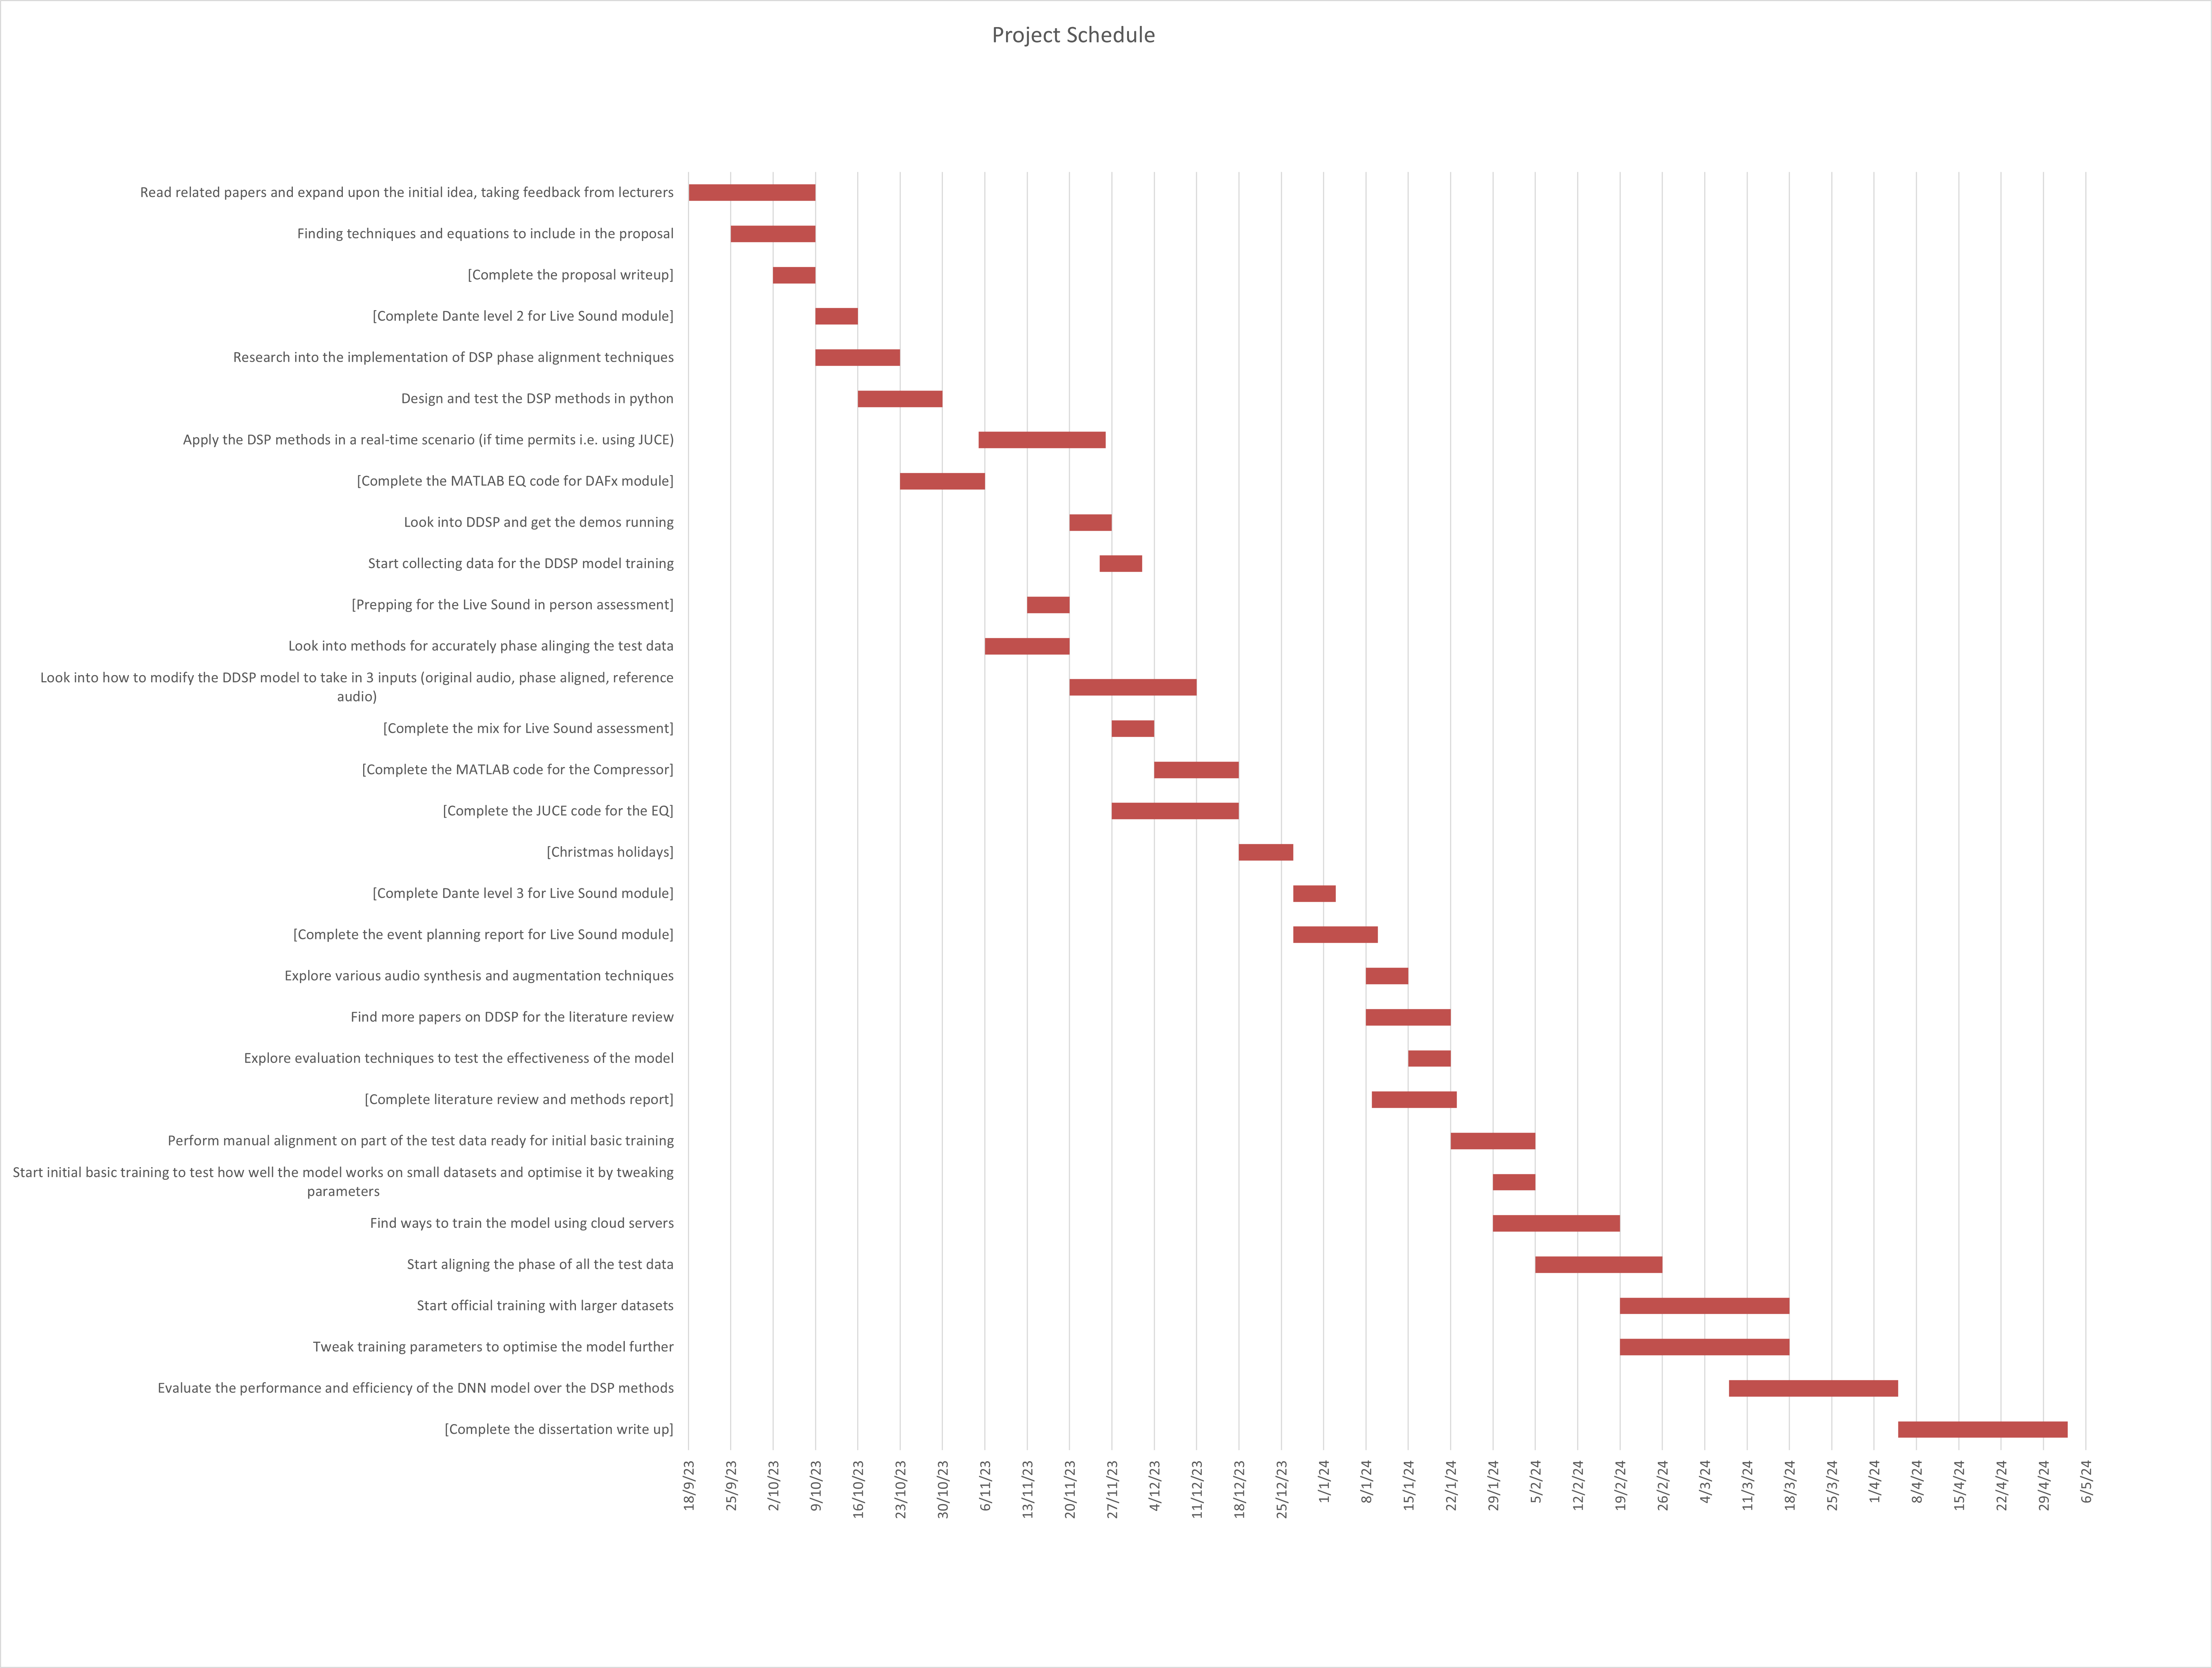
\includegraphics[width=0.95\linewidth]{Images/GANTT.png}
                \caption{Gantt Chart}
                \label{fig:gantt_chart}
            \end{figure}

        \end{landscape}

\end{appendices}

\end{document}